\documentclass[format=acmsmall, review=false,screen]{acmart}
\usepackage[T1]{fontenc}
\usepackage{tikz}
\usetikzlibrary{arrows.meta}

\begin{document}

		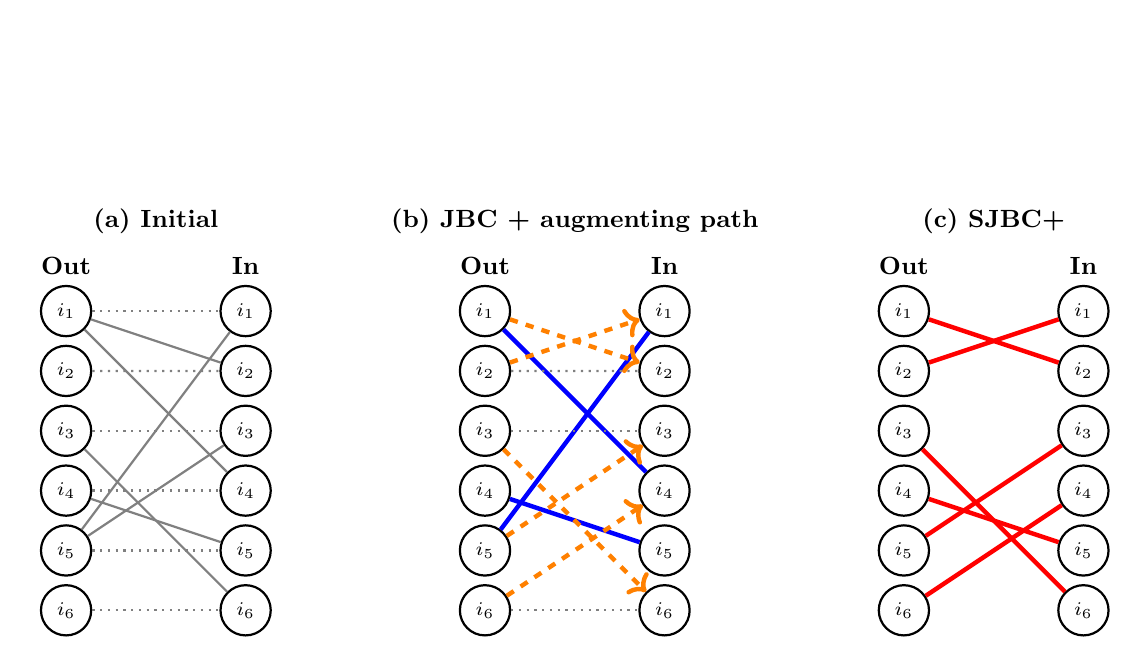
\begin{tikzpicture}[scale=0.38, thick,
	every node/.style={draw, circle, minimum size=0.35cm, font=\scriptsize}]

	% ============ PANEL (a): ALL SELF-LOOPS ============

	\def\xa{0}

	% Left column
	\foreach \i/\y in {1/10, 2/8, 3/6, 4/4, 5/2, 6/0} {
		\node (A_L\i) at (\xa, \y) {$i_\i$};
	}
	% Right column
	\foreach \i/\y in {1/10, 2/8, 3/6, 4/4, 5/2, 6/0} {
		\node (A_R\i) at (\xa+6, \y) {$i_\i$};
	}

	% All self-loops (dotted gray)
	\draw[dotted, gray, thick] (A_L1) -- (A_R1);
	\draw[dotted, gray, thick] (A_L2) -- (A_R2);
	\draw[dotted, gray, thick] (A_L3) -- (A_R3);
	\draw[dotted, gray, thick] (A_L4) -- (A_R4);
	\draw[dotted, gray, thick] (A_L5) -- (A_R5);
	\draw[dotted, gray, thick] (A_L6) -- (A_R6);

	\draw[ gray, thick] (A_L1) -- (A_R2);		
	\draw[ gray, thick] (A_L1) -- (A_R4);		
	\draw[ gray, thick] (A_L3) -- (A_R6);		
	\draw[gray, thick] (A_L5) -- (A_R3);		
	\draw[gray, thick] (A_L5) -- (A_R1);		
	\draw[ gray, thick] (A_L4) -- (A_R5);		
	% Labels
	\node[draw=none, font=\small] at (\xa, 11.5) {\textbf{Out}};
	\node[draw=none, font=\small] at (\xa+6, 11.5) {\textbf{In}};
	\node[draw=none, font=\small] at (\xa+3, 13) {\textbf{(a) Initial}};

	% ============ PANEL (b): AFTER JBC + AUGMENTING PATH ============

	\def\xb{14}

	% Left column
	\foreach \i/\y in {1/10, 2/8, 3/6, 4/4, 5/2, 6/0} {
		\node (B_L\i) at (\xb, \y) {$i_\i$};
	}
	% Right column
	\foreach \i/\y in {1/10, 2/8, 3/6, 4/4, 5/2, 6/0} {
		\node (B_R\i) at (\xb+6, \y) {$i_\i$};
	}

	% JBC matching (blue, thick)
	\draw[blue, ultra thick] (B_L1) -- (B_R4);
	\draw[blue, ultra thick] (B_L4) -- (B_R5);
	\draw[blue, ultra thick] (B_L5) -- (B_R1);

	% Self-loops (dotted gray)
	\draw[dotted, gray, thick] (B_L2) -- (B_R2);
	\draw[dotted, gray, thick] (B_L3) -- (B_R3);
	\draw[dotted, gray, thick] (B_L6) -- (B_R6);

	% Augmenting path (dashed orange)
	\draw[->, orange, dashed, ultra thick] (B_L2) -- (B_R1);
	\draw[->, orange, dashed, ultra thick] (B_L5) -- (B_R3);
	\draw[->, orange, dashed, ultra thick] (B_L3) -- (B_R6);
	\draw[->, orange, dashed, ultra thick] (B_L6) -- (B_R4);
	\draw[->, orange, dashed, ultra thick] (B_L1) -- (B_R2);

	% Labels
	\node[draw=none, font=\small] at (\xb, 11.5) {\textbf{Out}};
	\node[draw=none, font=\small] at (\xb+6, 11.5) {\textbf{In}};
	\node[draw=none, font=\small] at (\xb+3, 13) {\textbf{(b) JBC + augmenting path}};

	% ============ PANEL (c): OPTIMAL MATCHING ============

	\def\xc{28}

	% Left column
	\foreach \i/\y in {1/10, 2/8, 3/6, 4/4, 5/2, 6/0} {
		\node (C_L\i) at (\xc, \y) {$i_\i$};
	}
	% Right column
	\foreach \i/\y in {1/10, 2/8, 3/6, 4/4, 5/2, 6/0} {
		\node (C_R\i) at (\xc+6, \y) {$i_\i$};
	}

	% Optimal matching (red, thick)
	\draw[red, ultra thick] (C_L1) -- (C_R2);
	\draw[red, ultra thick] (C_L2) -- (C_R1);
	\draw[red, ultra thick] (C_L3) -- (C_R6);
	\draw[red, ultra thick] (C_L4) -- (C_R5);
	\draw[red, ultra thick] (C_L5) -- (C_R3);
	\draw[red, ultra thick] (C_L6) -- (C_R4);

	% Labels
	\node[draw=none, font=\small] at (\xc, 11.5) {\textbf{Out}};
	\node[draw=none, font=\small] at (\xc+6, 11.5) {\textbf{In}};
	\node[draw=none, font=\small] at (\xc+3, 13) {\textbf{(c) SJBC+}};

\end{tikzpicture}

\end{document}